\documentclass{article}

\usepackage{pgfplots}


\begin{document}

\pgfplotsset{
compat=1.8,
colormap={whitered}{color(0cm)=(white); color(1cm)=(orange!75!red)}
}

\pgfmathsetseed{42}

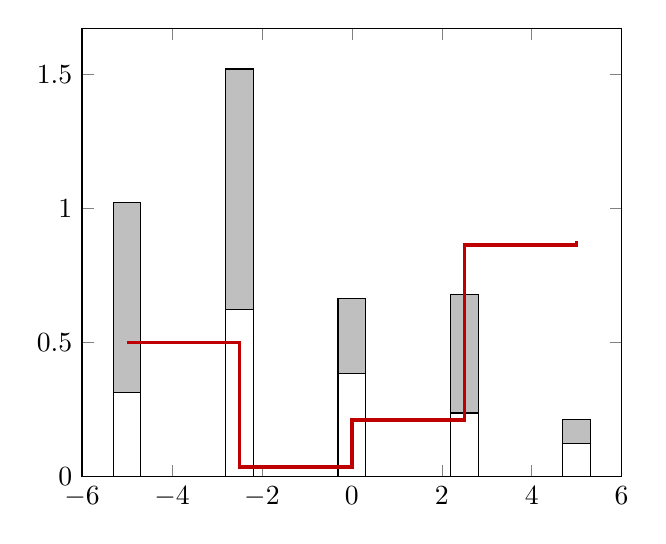
\begin{tikzpicture}
\begin{axis}[
    samples=5,
    ybar stacked,
    ymin=0,
    set layers
]
\addplot +[white, draw=black] {rnd};
\addplot +[gray!50, draw=black] {rnd};
\addplot [
    very thick, red!75!black,
    const plot,
    stack plots=false,
    on layer=axis foreground
] {rnd};
\end{axis}
\end{tikzpicture}
\end{document}


\documentclass{standalone}

\usepackage{tikz}
\usepackage{pgfplots}
\pgfplotsset{compat=newest}

\pgfplotstableread{
1   19.178  26.027  8.219   6.849   39.726 1
2   54.795  21.918  4.110   6.849   12.329 1
3   28.767  16.438  6.849   8.219   39.726 1
4   63.014  2.740   2.740   2.740   28.767 2
5   90.411  1.370   6.849   0.000   1.370  2
6   15.068  2.740   16.438  8.219   57.534 2
7   67.123  0.000   0.000   0.000   32.877 3
8   72.603  6.849   5.479   0.000   15.068 3
9   56.164  12.329  6.849   4.110   20.548 3
10  50.685  4.110   8.219   1.370   35.616 3
}\datatable

\begin{document}
\makeatletter
\begin{tikzpicture}
%\tracingmacros=2 \tracingcommands=2
\begin{axis}[
    ybar stacked
]

\addplot table[x index=0,y index=1] \datatable;
\addplot table[x index=0,y index=2] \datatable;
\addplot table[x index=0,y index=3] \datatable;
\addplot table[x index=0,y index=4] \datatable;
\addplot [stack plots=false] table[x index=0,y index=5] \datatable;
\legend{Far,Near,Here,There,NotThere}
\end{axis}
\end{tikzpicture}
\end{document}
